\documentclass[12pt]{article}
\usepackage{geometry}
\usepackage{textcomp}
\usepackage{enumitem}
\usepackage{amsmath} 
\usepackage{graphicx}
% \usepackage{showframe}


% chktex-file 44


\usepackage{listings}
\usepackage{color}

\definecolor{dkgreen}{rgb}{0,0.6,0}
\definecolor{gray}{rgb}{0.5,0.5,0.5}
\definecolor{mauve}{rgb}{0.58,0,0.82}

\lstset{frame=tb,
  language=python,
  aboveskip=3mm,
  belowskip=3mm,
  showstringspaces=false,
  columns=flexible,
  basicstyle={\small\ttfamily},
  numbers=none,
  numberstyle=\tiny\color{gray},
  keywordstyle=\color{blue},
  commentstyle=\color{dkgreen},
  stringstyle=\color{mauve},
  breaklines=true,
  breakatwhitespace=true,
  tabsize=3
}

\geometry{
  left=1in,
  right=1in,
  top=1in,
  bottom=1in,
}

\begin{document}

\setcounter{section}{-1}

\title{Machine learning approaches for \\ Telco Customer Churn}
\author{UNIVERSITY OF VERONA \\ Reza Ahmadi (VR510067)}
\date{June, 2024}
\maketitle
\vspace{1cm}



\begin{figure}[htbp]
  \centering
  
\includegraphics[width=0.5\textwidth]{assets/uni_logo.png}
\end{figure}


\begin{figure}[htbp]
  \centering
  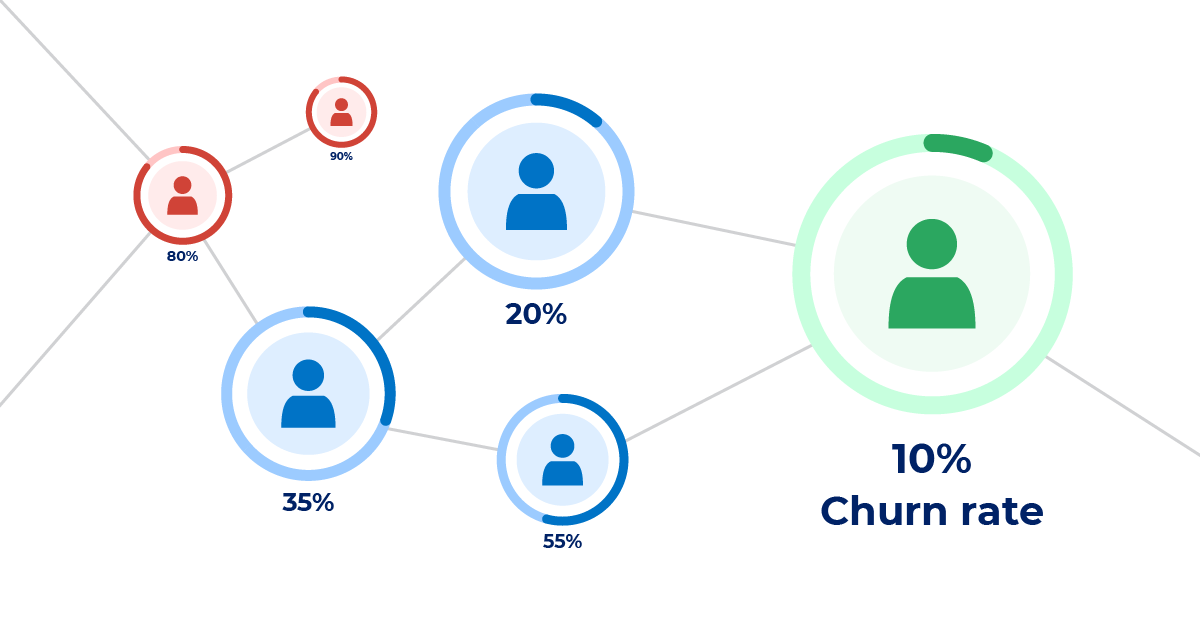
\includegraphics[width=\textwidth]{assets/first_page.png}
\end{figure}

\newpage

\section{Preface}

I am delighted to present this report detailing the exploration and application of machine learning techniques to analyze Telco customer churn data. This project represents a significant endeavor, aiming to uncover insights that can inform business strategies and enhance customer retention efforts.\\
I would like to express my sincere gratitude to Professors Vittorio Murino, Cigdem Beyan, and Andrea Avogaro for their invaluable guidance and support throughout this course and project. Their expertise and encouragement have been instrumental in shaping my understanding of machine learning concepts and methodologies.
\newpage

\tableofcontents

\newpage


\section{Introduction}
Telco Systems, a global telecom leader with 40+ years of experience in the design and development of high-performance network communications solutions.
They have released a dataset with various attributes about some of their users, and it contains an important field that is Churn.\\
We have worked with this dataset in this project in order to apply some machine learning approach and discover more information from this data set.

\section{About Dataset}
Data set is already avaialbe on the kaggle.

\subsection{Download dataset}
In order to download dataset, we should surfe this link:\\
https://www.kaggle.com/datasets/blastchar/telco-customer-churn/data

\subsection{Dataset information}
\begin{itemize}
  \item Customers who left within the last month, the column is called Churn
  \item Services that each customer has signed up for phone, multiple lines, internet, online security, online backup, device protection, tech support, and streaming TV and movies
  \item Customer account information, how long they've been a customer, contract, payment method, paperless billing, monthly charges, and total charges
  \item Demographic info about customers gender, age range, and if they have partners and dependents
\end{itemize}

\newpage
\subsection{Explore dataset}
The raw data contains 7043 rows (customers) and 21 columns (features).
List of columns that are already avaialbe in the dataset:
% \begin{itemize}
%   \item customerID
%   \item gender
%   \item SeniorCitizen: Whether the customer is a senior citizen or not (1, 0)
%   \item Partner: Whether the customer has a partner or not (Yes, No)
%   \item Dependents: Whether the customer has dependents or not (Yes, No)
%   \item Tenure: Number of months the customer has stayed with the company
%   \item PhoneService: Whether the customer has a phone service or not (Yes, No)
%   \item MultipleLines: Whether the customer has multiple lines or not (Yes, No, No phone service)
%   \item InternetService: Customer's internet service provider (DSL, Fiber optic, No)
%   \item OnlineSecurity: Whether the customer has online security or not (Yes, No, No internet service)
%   \item OnlineBackup: Whether the customer has online backup or not (Yes, No, No internet service)
%   \item DeviceProtection: Whether the customer has device protection or not (Yes, No, No internet service)
%   \item TechSupport: Whether the customer has tech support or not (Yes, No, No internet service)
%   \item StreamingTV\@: Whether the customer has streaming TV or not (Yes, No, No internet service)
%   \item StreamingMovies: Whether the customer has streaming movies or not (Yes, No, No internet service)
%   \item Contract: The contract term of the customer (Month-to-month, One year, Two year)
%   \item PaperlessBilling: Whether the customer has paperless billing or not (Yes, No)
%   \item PaymentMethod: The customer's payment method (Electronic check, Mailed check, Bank transfer (automatic), Credit card)
%   \item MonthlyCharges: The amount charged to the customer monthly
%   \item TotalCharges: The total amount charged to the customer
%   \item Churn: Whether the customer churned or not (Yes or No)
% \end{itemize}


\begin{table}[ht]
  \centering
  \small
  \begin{tabular}{|l|l|l|}
    \hline
    \textbf{Field} & \textbf{Values} & \textbf{Description} \\
    \hline
    customerID & String & Unique identifier \\
    gender & Male, Female & Gender \\
    SeniorCitizen & 1, 0 & Senior citizen status \\
    Partner & Yes, No & Has a partner \\
    Dependents & Yes, No & Has dependents \\
    Tenure & Numeric & Months with company \\
    PhoneService & Yes, No & Has phone service \\
    MultipleLines & Yes, No, No phone & Has multiple lines \\
    InternetService & DSL, Fiber optic, No & Internet service provider \\
    OnlineSecurity & Yes, No, No internet & Has online security \\
    OnlineBackup & Yes, No, No internet & Has online backup \\
    DeviceProtection & Yes, No, No internet & Has device protection \\
    TechSupport & Yes, No, No internet & Has tech support \\
    StreamingTV & Yes, No, No internet & Has streaming TV \\
    StreamingMovies & Yes, No, No internet & Has streaming movies \\
    Contract & Month-to-month, One year, Two year & Contract term \\
    PaperlessBilling & Yes, No & Paperless billing \\
    PaymentMethod & Electronic, Mailed, Bank transfer, Credit card & Payment method \\
    MonthlyCharges & Numeric & Monthly charges \\
    TotalCharges & Numeric & Total charges \\
    Churn & Yes, No & Churn status \\
    \hline
  \end{tabular}
  \caption{Description of Fields}
  \end{table}
  

\newpage
\section{Open Dataset in Enviroment}
In order to produce a data frame from data, we have used the Pandas library, below code can satisfy our expectation.
\begin{lstlisting}
  import pandas as pd
  df = pd.read_csv("data/WA_Fn-UseC_-Telco-Customer-Churn.csv")
  print("Shape of datasset",df.shape)
  df.head()
  \end{lstlisting}
  It is clear that two first lines of the code are trying to import libraries and in the third line it is trying to open a CSV dataset and retain it as a data frame in a variable and then we have tried to show the results.

\section{Visualization}
In this part, we have tried to provide some visualization by charts in order to have better imagination from data.

\subsection{Discrete value fields}
The most useful type of charts for visualizing discrete values is pie charts. As we have seen in the 2.3 section we have many discrete fields, but we are going to visualize 9 of the most important.\\
The most important discrete fields seem:
\begin{itemize}
  \item Gender
  \item Internet Service
  \item Contract
  \item Paperless Billing
  \item PaymentMethod
  \item Churn
\end{itemize}
\vspace{1cm}
For producing these charts we are using matplot library, so we have written this code:



\newpage
\begin{lstlisting}
  import matplotlib.pyplot as plt

  print("Distribution of Some Interesting Discrete Features")
  
  # Define the data for each pie chart
  gender_counts = df['gender'].value_counts()
  internet_counts = df['InternetService'].value_counts()
  contract_counts = df['Contract'].value_counts()
  paperless_billing_counts = df['PaperlessBilling'].value_counts()
  payment_method_counts = df['PaymentMethod'].value_counts()
  churn_counts = df['Churn'].value_counts()
  
  # Create a figure with multiple subplots
  fig, axs = plt.subplots(2, 3, figsize=(15, 10))
  
  # Plot each pie chart in its corresponding subplot
  axs[0, 0].pie(gender_counts, labels=gender_counts.index, autopct='%1.1f%%', startangle=90)
  axs[0, 0].set_title('Gender')
  
  axs[0, 1].pie(internet_counts, labels=internet_counts.index, autopct='%1.1f%%', startangle=90)
  axs[0, 1].set_title('Internet Service')
  
  axs[0, 2].pie(contract_counts, labels=contract_counts.index, autopct='%1.1f%%', startangle=90)
  axs[0, 2].set_title('Contract')
  
  axs[1, 0].pie(paperless_billing_counts, labels=paperless_billing_counts.index, autopct='%1.1f%%', startangle=90)
  axs[1, 0].set_title('Paperless Billing')
  
  axs[1, 1].pie(payment_method_counts, labels=payment_method_counts.index, autopct='%1.1f%%', startangle=90)
  axs[1, 1].set_title('Payment Method')
  
  axs[1, 2].pie(churn_counts, labels=churn_counts.index, autopct='%1.1f%%', startangle=90)
  axs[1, 2].set_title('Churn Distribution')
  
  # Adjust layout
  plt.tight_layout()
  
  # Display the plot
  plt.show()  
  \end{lstlisting}
  \vspace{\baselineskip}
In the above code, first we have tried to import the Matplot library. Then the features for visualize are separated in each specific variables then we have defined a figure like 2 by 3 and 15 $\times$ 10 dimensions and on the remaining lines the data are passed to each position, and finally we have plotted charts.\\
The result is like the following figure.
\newline
\vspace{1cm}
\begin{figure}[htbp]
  \centering
  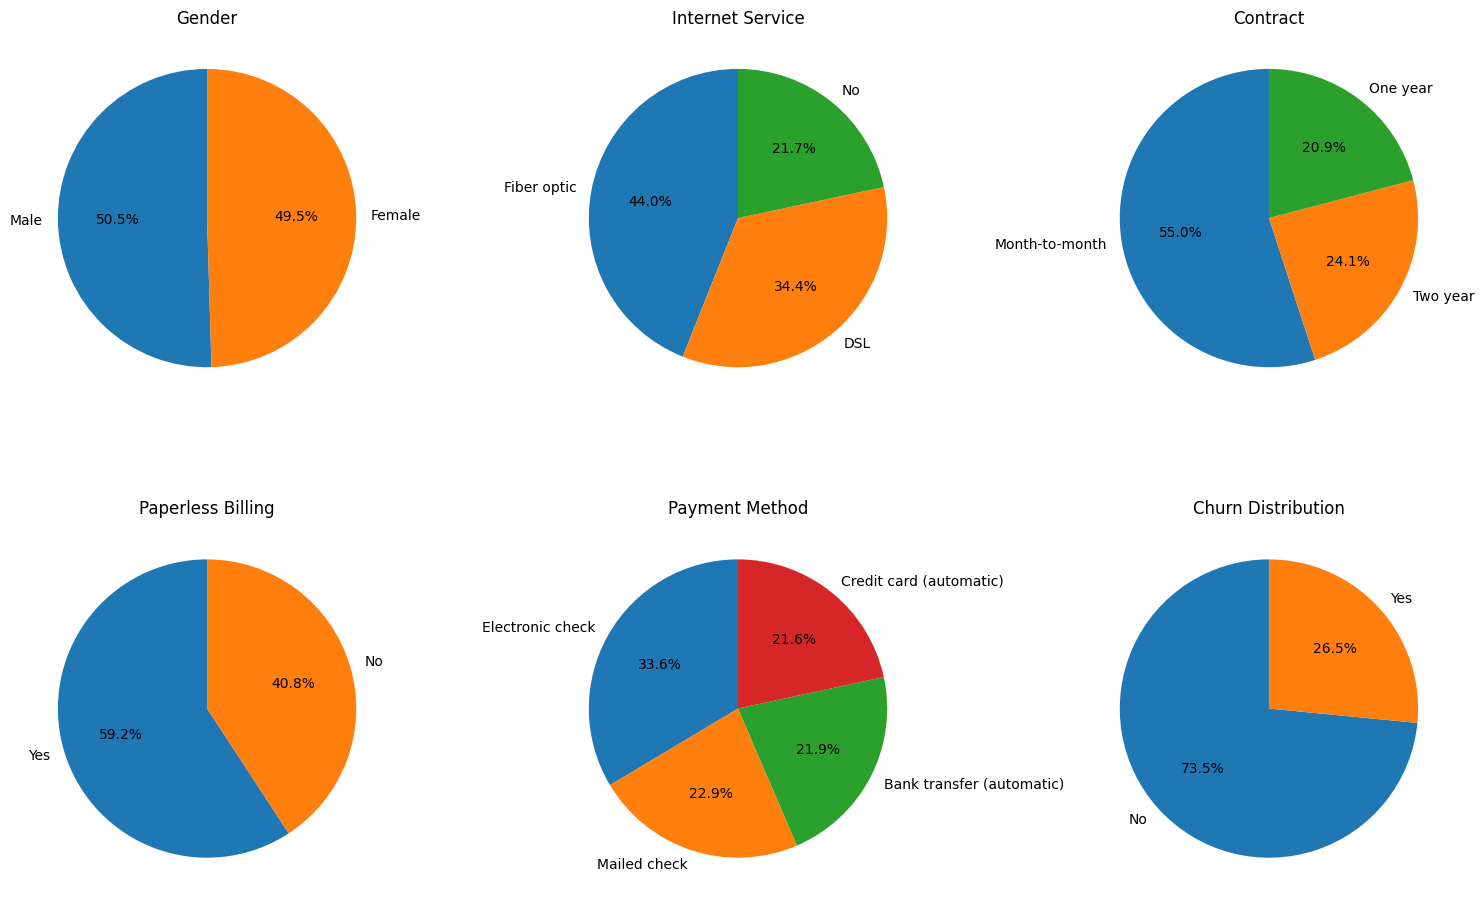
\includegraphics[width=\textwidth]{assets/distributatuons.png}
  \caption{Distributatuons of some discrete fields}
\end{figure}
\vspace{\baselineskip}
\newline
The most interesting pie chart is Churn Distribution. It is obvious that 26.5 percent of data are about the people that leave getting services from the company, but other users are still remaining.


\newpage
\subsection{Continues value fields}
One of the most important charts for visualizing continues value is Histograms, with this chart we can see the scattering of data by each specific unit.
As we have mentioned in the section 2.3 there are several continues value in the dataset, it seems the most important are:
\begin{itemize}
  \item Tenure
  \item Monthly Charges
  \item Total Charges
\end{itemize}
\vspace{1cm}
For visualize Histogram we are using Matplot library again, so the implementation is like this:

\vspace{1cm}

\begin{lstlisting}
  plt.figure(figsize=(8, 5))
  plt.hist(df['tenure'], bins=20, color='blue', edgecolor='black')
  plt.xlabel('Tenure')
  plt.ylabel('Frequency')
  plt.title('Histogram of Tenure')
  plt.grid(True)
  plt.show()
\end{lstlisting}
\vspace{\baselineskip}
In the represented code, a plot is defined with 8 $\times$ 5 dimensions, then tenure features from the dataset have passed and on the rest of the code we have defined just visualization properties.\\
The result of the code is a histogram chart like this:
\begin{figure}[htbp]
  \centering
  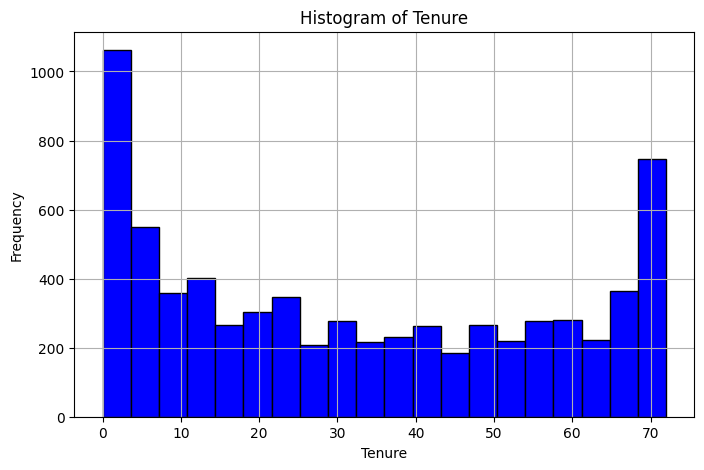
\includegraphics[width=0.6\textwidth]{assets/hist_tenure.png}
  \caption{Histogram of tenure}
\end{figure}
\vspace{\baselineskip}
\newline
With the first look we can find that the most of the users have joined the company early and less than 5 months and also the other segments are really loyal users.\\
\vspace{\baselineskip}
\newline
For Monthly Charges we have this part of code:

\vspace{1cm}

\begin{lstlisting}
  total_charges_data = df['MonthlyCharges'].astype('int')
  plt.figure(figsize=(8, 5))
  plt.hist(total_charges_data, bins=20, color='blue',edgecolor='black')
  plt.xlabel('Monthly Charges')
  plt.ylabel('Frequency')
  plt.title('Histogram of Monthly Charges')
  plt.grid(True)
  plt.show()
  \end{lstlisting}
  \vspace{\baselineskip}
  It is obvious that the above code is totally same with the tenure histogram, but we have changed the input data from the dataset to get Monthly Charges. Also in the first line we have changed the data type of the field to int.\\
  The result of the code is this chart:
  \begin{figure}[htbp]
    \centering
    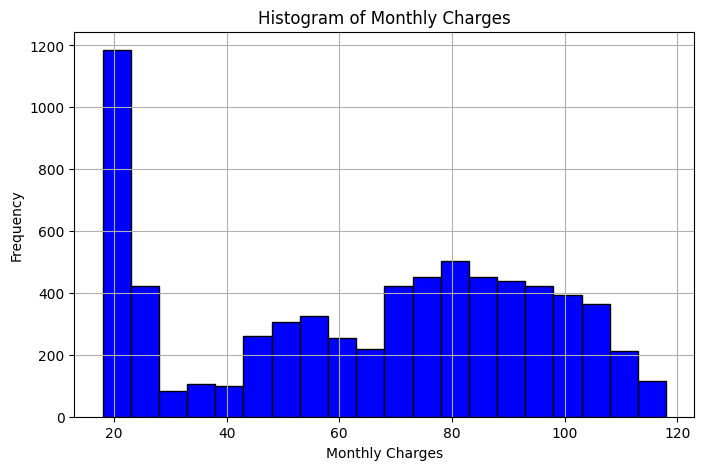
\includegraphics[width=0.6\textwidth]{assets/hist_monthly_charges.png}
    \caption{Histogram of Monthly Charges}
  \end{figure}
  \vspace{\baselineskip}
  \newline
  It is understandable from the above chart that the biggest segment of the users have 20 units of monthly charge.
  \vspace{\baselineskip}
  \newline
  For Total Charges we have exactly the same code with Monthly Charges with different input to Matplotlib. The code is like this:
  \newpage
  \begin{lstlisting}
    total_charges_data = df['TotalCharges'].replace(['', ' '], '0').astype('float').round(2).astype('int')
    plt.figure(figsize=(8, 5))
    plt.hist(total_charges_data, bins=20, color='blue',edgecolor='black')
    plt.xlabel('Total Charges')
    plt.ylabel('Frequency')
    plt.title('Histogram of Total Charges')
    plt.grid(True)
    plt.show()
    \end{lstlisting}
    Like Monthly Charges, we were have to change data type of Total Charges and replace empty columns with zero, and we have got this result: 
    \begin{figure}[htbp]
      \centering
      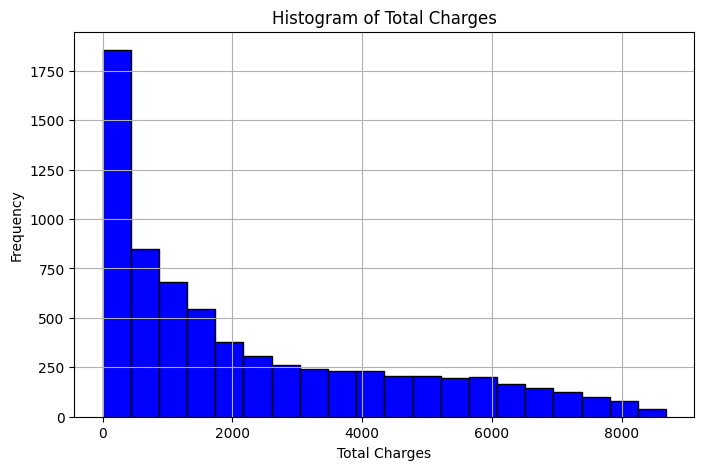
\includegraphics[width=0.6\textwidth]{assets/hist_total_charges.png}
      \caption{Histogram of Total Charges}
    \end{figure}
    \vspace{\baselineskip}
    \newline
    We have understood that most of the users have total charges below 2000 units.

\end{document}